% !TEX root = main.tex

% \addtocontents{toc}{\protect\newpage}
\secc{Design and implementation}

\ssecc{Get familiar with survival models}

\ssecc{Preprocess data}

As it was previously stated the data needs to be preprocessed before start training with it.
This steps are required because small changes can really help in reducing the time needed to
fit the model. Also, by normalizing the data and setting variance to 1 and mean to 0 the network
can converge faster.
~\cite{neural:efficient-backprop}

\sssecc{Image data}

The imaging data in the \Gls{PMHNK} contains 671 folders, each one with the scan of one patient. 
We also have the clinical information of 661 patients, although we do not have a \gls{CT} for
each of the clinical information patients. Through the intersection of each of the two data
sources we have 544 patients with both a \gls{CT} scan and the clinical information.

However, because there was a problem in the way the \gls{CT} scan was computed we only have
the tumour annotations for 509 of the 544 patients, so the data that we can use is reduced
again. \textbf{509} will be the final dataset size that will be used for the next 
steps.

For all the valid patients their directory structure is the same. They contain two folders,
one with all the original scan slices and the other with the slice's tumour mask annotations. 
All the slices are in \verb|.dcm| format.
For example if we have the patient \texttt{FHBO003} the structure can be seen in 
\autoref{fig:hnk-raw}.

\begin{figure}
  \centering
  \begin{minipage}{0.8\textwidth}
    \begin{Verbatim}[samepage=true]
      FHBO003
      ├── FHBO003           // Original scan
      │   ├── IMG0001.dcm
      │   ├── IMG0002.dcm
      │   ├── ...
      │   └── IMG0191.dcm
      └── FHBO003-MASS      // Annotated mask
      ├── IMG0001.dcm
      ├── IMG0002.dcm
      ├── ...
      └── IMG0191.dcm
    \end{Verbatim}
  \end{minipage}
    
  \caption{Original data directory structure \label{fig:hnk-raw}}
\end{figure}

Preprocessing the image data requires multiple steps:
\begin{enumerate}
  \item Select valid directories that follow the previously stated conditions
  \item Join all the \verb|.dcm| files into a 3D \verb|numpy| array
  \item Apply gaussian filter to mask image. This is done because the mask is manually annotated
        and usually each layer does not fit perfectly with the previous one. This way a smooth
        transition between layers is ensured.
  \item Get 3D bounding box containing the tumour.
  \item Slice original image and mask with the bounding box to extract the parts only containing
        the tumour. A single bounding box is obtained.
  \item Remove extreme values, if the value of the image is smaller than -1000 or bigger than
        400 this means that this are pixels usually outside of the scanner. This happens because
        the scanner has a circular field of view but a squared image is generated instead, so 
        all the pixels outside the circle are \emph{error pixels}.
  \item Apply mask to extracted image. Since the mask only contains 1s and 0s it's as easy 
        as \verb|image *= mask|.
  \item Resize the sliced image to a size of \( 64 \times 64 \times 64 \)
  \item Normalize image by setting mean = 0 and variance = 1. It's done in the following way:
  \begin{itemize}
    \item \verb|image -= mean(image)|
    \item \verb|image /= std(image)|
  \end{itemize}
  \item Rotate the image 3 times to get 4 different versions of the scan that can be used for 
        training as data augmentation.
\end{enumerate}

\begin{figure}
  \resizebox{\textwidth}{.7\textwidth}{
    \def\customimage{10em}
\begin{tikzpicture}[node distance = 2]
    \node (P-0) at (0, 0) {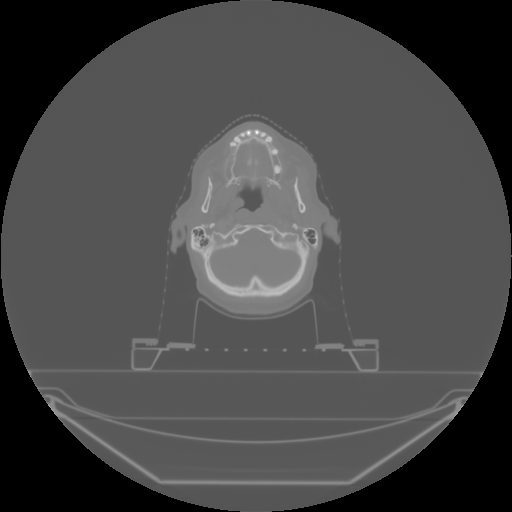
\includegraphics[width=\customimage]{images/preprocess/process_0}};
    \node [below = of P-0] (P-1) {
\includegraphics[width=\customimage]{images/preprocess/process_1}};

    \node [below = .2 of P-0] (text-0) {Scan};
    \node [below = .2 of P-1] (text-1) {Mask};
    
    \node [right = of P-1] (P-2-0) {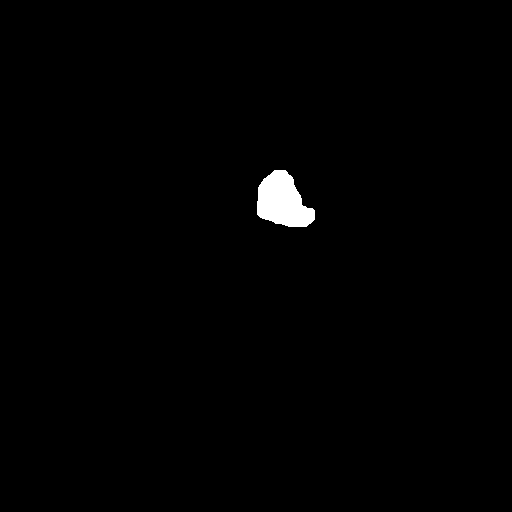
\includegraphics[width=\customimage]{images/preprocess/process_2_0}};
    \node [right = of P-2-0] (P-2-1) {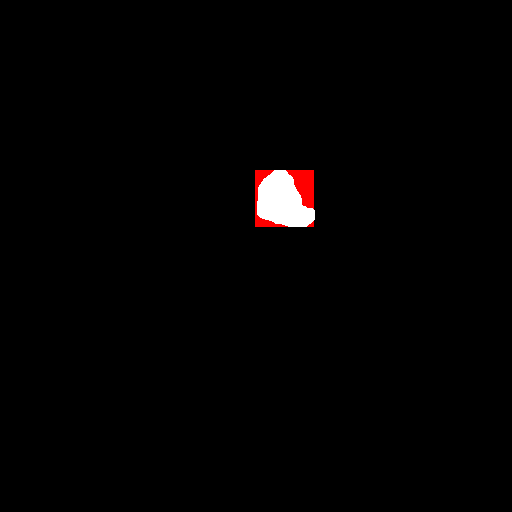
\includegraphics[width=\customimage]{images/preprocess/process_2_1}};
    \node [right = of P-2-1] (P-5) {
\includegraphics[width=\customimage]{images/preprocess/process_5}};
    
    \node [above = of P-2-1] (P-3) {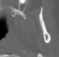
\includegraphics[width=\customimage]{images/preprocess/process_3}};
    \node [right = of P-3] (P-4) {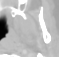
\includegraphics[width=\customimage]{images/preprocess/process_4}};

    \node [right = .5 of P-5, circle, draw] (prod) { \Large \( \times \) };
    
    \node [below = of P-5] (P-6) {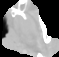
\includegraphics[width=\customimage]{images/preprocess/process_6}};
    \node [left = of P-6] (P-7) {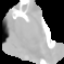
\includegraphics[width=\customimage]{images/preprocess/process_7}};
    \node [left = of P-7] (P-8) {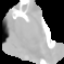
\includegraphics[width=\customimage]{images/preprocess/process_8}};

    \node [below = .2 of P-6] { \( 59 \times 57 \) px};
    \node [below = .2 of P-7] { \( 64 \times 64 \) px};
    \node [below = .2 of P-8] { \( 64 \times 64 \) px};

    \draw [-latex] (P-0) -- (P-3);
    \draw [-latex] (P-3) -- (P-4) node[midway, below, align=center] {Remove \\ extreme \\ values};
    \draw [-latex] (P-4) -| (prod);

    \draw [-latex] (P-1) -- (P-2-0) node[midway, below, align=center] {Gaussian \\ filter};
    \draw [-latex] (P-2-0) -- (P-2-1) node[midway, below, align=center] {Bounding \\ box};
    \draw [-latex] (P-2-1) -- (P-3) node[midway, right, align=center] {Slice};
    \draw [-latex] (P-2-1) -- (P-5) node[midway, below, align=center] {Slice};
    \draw [-latex] (P-5) -- (prod);

    \draw [-latex] (prod) |- (P-6) node[near end, below, align=center] {Apply \\ mask};
    \draw [-latex] (P-6) -- (P-7) node[midway, below, align=center] {
        Resize \\ \( 64 \times 64 \times 64 \)
    };

    \draw [-latex] (P-7) -- (P-8) node[midway, below, align=center] {Normalize};

\end{tikzpicture}
  }

  \caption{Image pre-process pipeline \label{fig:preprocess}}

  \it
  In this example the process is shown for a 2D image, all the pictures are being resized to 
  have the same size so the steps can be appreciated. The normalization step is not shown as is
  since setting a mean of 0 and variance of 1 produces an invalid \acrshort{PNG} image, but still valid
  for \gls{ML} purposes.
\end{figure}

\sssecc{Scalar data}

There are two types of scalar data:
\begin{itemize}
  \item Clinical information
  \item Radiomic features extracted from the image, regarding tumour shape, intensity, volume...
\end{itemize}

The clinical information should be anonymized as much as possible and especially if it's going
to be outside \gls{UHN}, the network of hospitals where this project is being developed.
Since this is the case, as the training will be done at \gls{CC} cluster, the unnecessary fields
are removed and only the ones that are being used are kept. Moreover, removing the unused fields
is helpful when using the data.

Originally, the clinical information provides 36 different fields. From this fields only the 
following ones are kept:
\begin{itemize}
  \item ID
  \item Age
  \item Sex
  \item Survival event, this one needs to be negated since, in the provided event, \verb|event = 1|
        means survival, but in our survival model this means death. 
  \item Survival time
\end{itemize}

The radiomic features can be extracted directly with the \emph{PyRadiomics}
\cite{medical:py-radiomics} package, but in this case they have been already extracted and stored
in a single file so we can reuse them. These features should be normalized before start training,
because otherwise the network may never converge, which indeed it happened. 

For this normalization to be valid the mean and the standard deviation is obtained only from 
the train samples. These are different for each feature because not all the features need to 
be normalized in the same way. Afterwards, the normalization is applied to both the train 
and test samples. The mean for the test samples is never obtained, because, otherwise, the
model could have \gls{leakage}. 


\sssecc{Pair generation}

\ssecc{Build shallow siamese network}

\ssecc{Build scalar only siamese network}

\ssecc{Build deeep siamese network}

